\chapter{Implementation}
\label{cha:impl}

In this chapter I will go through the entire process detailing how I go from a raw dataset, all the way to being displayed with Leaflet.

\section{Pre-Processing}

Figure \ref{bbdatatable} shows the raw format of the Britain Breathing dataset. There are a few procedures that need doing before it can be used in a hotspot identification algorithm. Before I had a web page running with the capability of displaying geographical data I relied on Tableau to visualise and alter all datasets.\\ 

The Britain Breathing dataset in its raw format contained entries from all over the world. I could have decided to leave them on as I could centre the map on the UK so only those who were curious enough to pan around the rest of the globe would see these extra points. But that's more of a novel thing. At the time of pre-processing, I thought the extra points might affect some of the hotspot algorithm calculations such as global averages so I decided to remove all points that are not on mainland UK or in Northern and the Republic of Ireland.\\

\begin{figure}[H]
\begin{center}
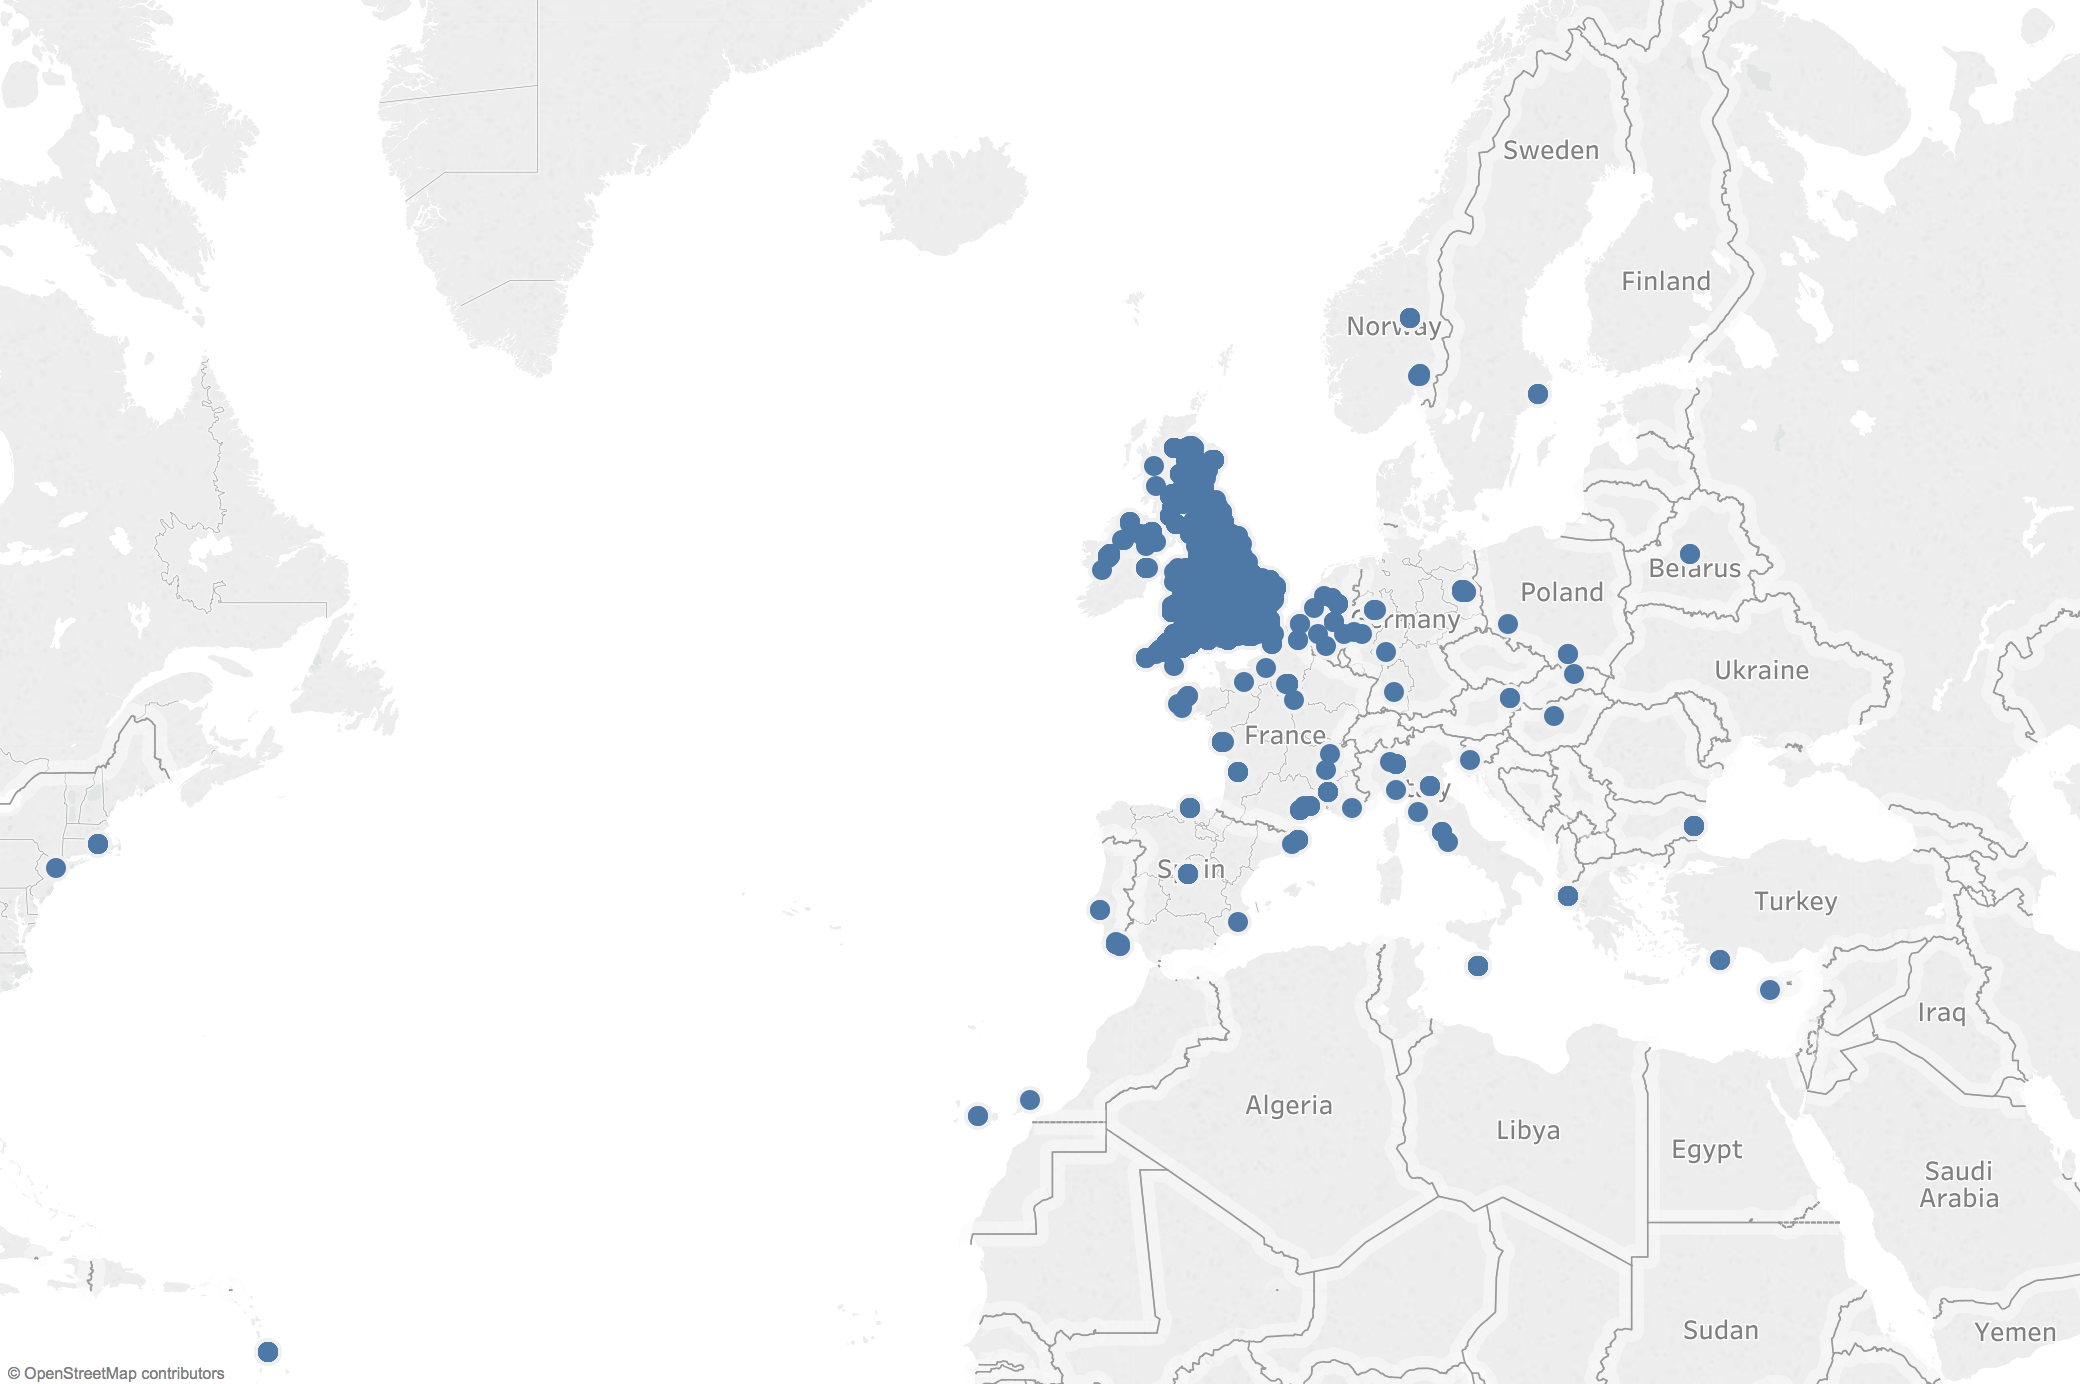
\includegraphics[width=0.75\textwidth]{tableuaeverywhere}
\caption{Britain Breathing dataset before processing}
\label{fig:RTv1}
\end{center}
\end{figure}

Approximately 2.7\% of entries had a null value for one of the attributes. 96\% of these nulls were  whether or not the user had existing hay fever or asthma, I decided to remove each of these records entirely, I could also have decided set the attribute to 0 or 1 but I wanted to avoid fabricating data to keep any conclusions made using the data valid.\\

Whilst using Tableau to visualise the data in the early stages of development I noticed there were a few clusters of points in virtually the same place. For example, there is a user in the north of Scotland who used the app at times multiple times a day to record her allergy symptoms. This resulted a fairly large set of results for a very sparsely populated area. I decided to remove most of the results for this person as the area was identified as a hotspot. I think there could be arguments for keeping the data but I don't think that allowing one person's enthusiasm to track her allergy problems makes sense for a project aimed at producing results that could be used to aid research.\\

Once the data has been improved from its raw format, it is stored on the server as a .JSON file. I decided against using a database to store my datasets as I wanted to avoid having to convert to and from JSON. The end application ended up being rather CPU intensive so this decision turned out very well.

\subsection{Road Traffic}

The Road Traffic dataset in its raw format was far from being usable.\\

As you can see from figure \ref{fig:rt} the first version of the Road Traffic dataset was way too dense. I needed the dataset to be able to be displayed with the heatmap generated from the Britain Breathing dataset to be visible behind the Road Traffic data in order to compare the two. There were too many roads of very short spans cluttering the view of the heatmap.\\

\begin{figure}[H]
\begin{center}
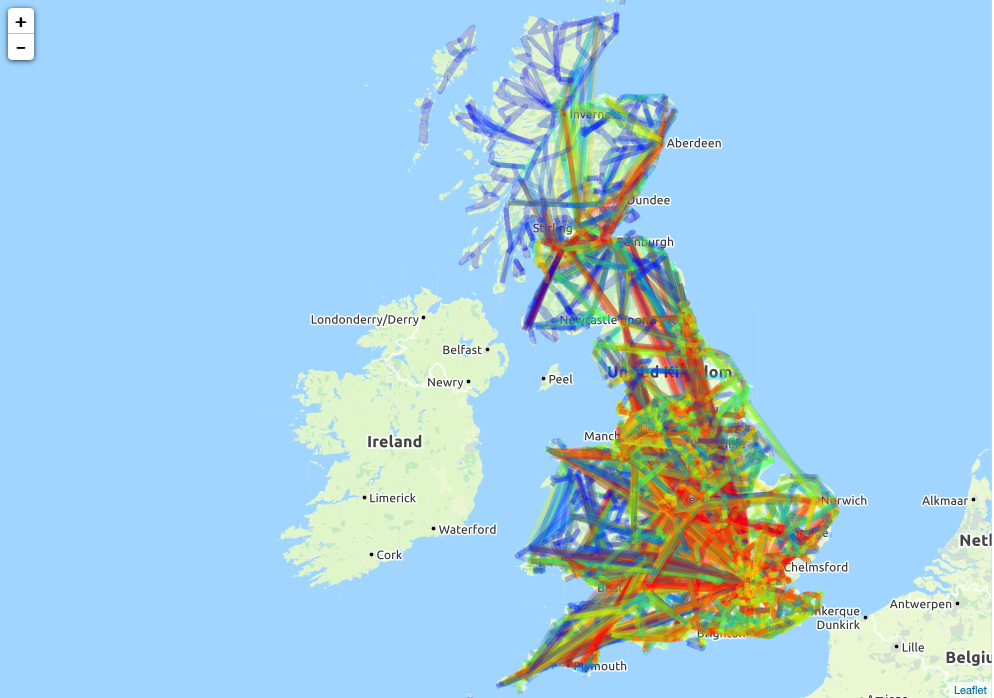
\includegraphics[width=0.75\textwidth]{RoadTrafficv1}
\caption{First attempt at displaying the Road Traffic data. There's a bit much going on here.}
\label{fig:rt}
\end{center}
\end{figure}

Upon zooming in and inspecting the data I also found that some roads were stored incorrectly in the dataset. Around 10 roads were stored as having their junction before and junction after being the ends of the road. Roads like the A1 can be as long as 396 miles so errors can cause big problems \cite{longestRoad}. In the case of the A1, the entire road was displayed as a deep red indicating a high volume of traffic. For the majority of the A1, this would be true but there are areas of the road that are not particularly busy so they're being wrongly represented. \\

I created a java program to process the data before being stored on the server. Java was chosen purely because I have most experience with it and I knew exactly how to read and write files, making it a good choice for pre-processing the Road Traffic data. For each entry, counts are discarded if the length of the distance between the junction before and the junction after is longer than 200km or if the road is shorter than 5km and has a density in the lower 5\% of the data. Removing the smaller roads like this removes the mess of small roads with negligible traffic in places like the north of Scotland. These roads don't provide much information and therefore do not help to find hotspots, they just make the map look cluttered.\\

\subsection{Analysis Field}
\label{sec:anal}

The Britain Breathing dataset has many attributes that are relevant to allergy symptoms.\\

Figure \ref{table:bbdata} : Britain Breathing Dataset Allergy Related Attributes. 13 attributes removed for simplicity.\\\label{table:bbdata}
\begin{tabular}{|c|c|c|c|}\hline\hline
Attribute&Represents&Range&Range Description\\\hline
how\_feeling&General well-being of the person&0..2&0 Best, 2 Worst\\
breathing&Condition of lungs and trachea&0..2&0 Best, 2 Worst\\
eyes&Condition of the eyes&0..2&0 Best, 2 Worst\\
nose&Condition of the nose&0..2&0 Best, 2 Worst\\
hayfever&Suffers from hay fever&0..1&0 no, 1 yes\\
asthma&Suffers from asthma&0..1&0 no, 1 yes\\
taken\_meds\_today&Taken allergy medication&0..1&0 no, 1 yes\\\hline\hline
\end{tabular}

All of the attributes in Figure \ref{table:bbdata} contribute to the overall severity of a persons allergy symptoms on any given day. In order to use with hotspot identification algorithms, I need a single attribute that is a summary of the others. I need to combine them all into one value that can be used to score a certain records Allergy Score, or more generically to fit the Road Traffic dataset too, the Analysis Field.\\

In the development of the Analysis Field for the Britain Breathing dataset, I made some initial judgements and then adjusted the parameters with some trial and improvement. The Analysis field needs to be a summary of the others. Keeping this in mind, I assigned a high priority to the how\_feeling attribute as it itself is a summary of the persons general allergy related feeling. I then assigned breathing, nose and eyes with roughly similar weightings. I used the taken\_medication\_today as a multiplier for the breathing, nose and eye symptoms using the logic that if a person has taken their medication and is still suffering, then they should score higher than someone with the same values for the other attributes but has not taken their medication. hayfever and asthma attributes are used, but do not have much of an effect on the Analysis Field.\\

\begin{myequation2}%
Analysis Field (AF) = 2*(how\_feeling*(0.5*nose + 0.3*eyes + 0.3*breathing))
\end{myequation2}
\begin{myequation2}%
+ (taken\_meds\_today*(nose + eyes + breathing)) + asthma + hayfever
\end{myequation2}

The above formula is used to calculate the Analysis field in the final version of Inhale. It seems to work well, I'm happy it uses a wide spread of attributes but still focuses on the main four; how\_feeling, nose, breathing and eyes.\\

The Analysis field for the Road Traffic dataset was simpler. To keep the field relevant to allergies, I decided to focus on the emissions from vehicles on that road per hour. At first I simply found that the average $CO_2$ emissions for a combustion engine vehicle was 411 g/mile or 274g/km and I multiplied the total traffic count by this value \cite{trafficemiss}. The traffic counts were not anywhere near perfectly distributed. Different roads had very different distributions of vehicle types. For example, the two main corridors between the North and South of England, the M6 on the East and the A1 on the West both had far higher percentages of HGV type vehicles than average.\\

With the disparity in vehicle distribution in mind, I found the average vehicle emissions for each vehicle type instead. Then simply created the Analysis Field as below.

\begin{myequation2}%
Analysis Field (AF) = \sum_{vt=1}^n VehicleCount * VehicleTypeEmissions
\end{myequation2}

As previously mentioned, the dataset is not entirely consistent with its junctions before and after the counting point. Ideally, I'd use the vehicle emissions per km and multiply that by the distance between the junction before and after to get a total emission value for the vehicle. Not only would this not be possible due to the problems in the dataset, but it would also produce useless results. It doesn't matter how far a vehicle has travelled on its way to you, only the distance it has travelled in a small radius around you should be considered as this is the area in which its emissions can reach affect you.\\

As a compromise, I simply used the g/km value without taking into account the actual number of km used. This could maybe be improved by calculating the distance of the road that is within x km of the user.

\section{Heatmap Generation}

Once the data is in a useable format and condition, I need to display that data on a map. In this section will explain the steps taken to get to point where I have a allergy symptom hotspot represented as a heatmap using Leaflet.\\

The Britain Breathing JSON file is loaded from the server. An instance of a HotspotArray is instantiated with parameters including x and y values for the dimension of the desired map resolution. The resolution values are used to create a two dimensional array with sizes [x][y]. This array is used to divide the area of the UK into distinct square areas. See figure \ref{fig:hh} for a small scale example.

\begin{figure}[H]
\begin{center}
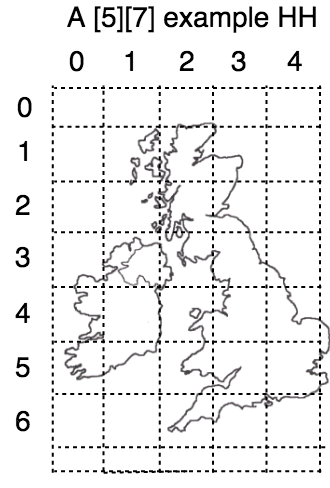
\includegraphics[width=0.4\textwidth]{hh5x7}
\caption{A [5][7] resolution example}
\label{fig:hh}
\end{center}
\end{figure}

By default, I used a 500 by 500 resolution as I found this gives enough of a resolution so that you can't see the square boundaries at any zoom level but also keeps the map easy to use in calculations. The alternative here would have been to use something like the UK Council boundaries, but I didn't like how they looked on the map. This was mainly due to the fact that dividing the map by Councils meant that you don't get precise enough information on specific allergy symptoms hotspots. A hotspot in a City such as Inverness would cause a massive area including tiny three or four house villages in the middle of the Scottish highlands to be indicated as being a "hotspot".\\

For each entry in the processed dataset;

\begin{enumerate}
    \item Add entry to the Hotspot Array. The latitude and longitude of the entry is used to map to an index in the array. For example, a location in the top left of the map would map to [0][0], bottom right would map to [499][499] etc. 
    \item If there is already a value in the Hotspot Array, add to the total count and update the average for the square area. Otherwise, add to the total count and calculate average.
\end{enumerate}

The next step after filling the Hotspot Array with the data is to do some hotspot identification.

\subsection{Spatial Autocorrelation}

Determining if an area is a hotspot or not can be done using Spatial Autocorrelation (SA). SA is a way of giving a numerical value to the degree of which an area is similar to nearby areas \cite{autocor} . A high positive value indicates that an area has a statistically significant value when compared to its neighbours and should be indicated as a hotspot. A low positive or negative value indicates that it is likely that the value is randomly clustered. A high negative value shows a cluster of low values. See Figure \ref{fig:autocor2}\\

\begin{figure}[H]
\begin{center}
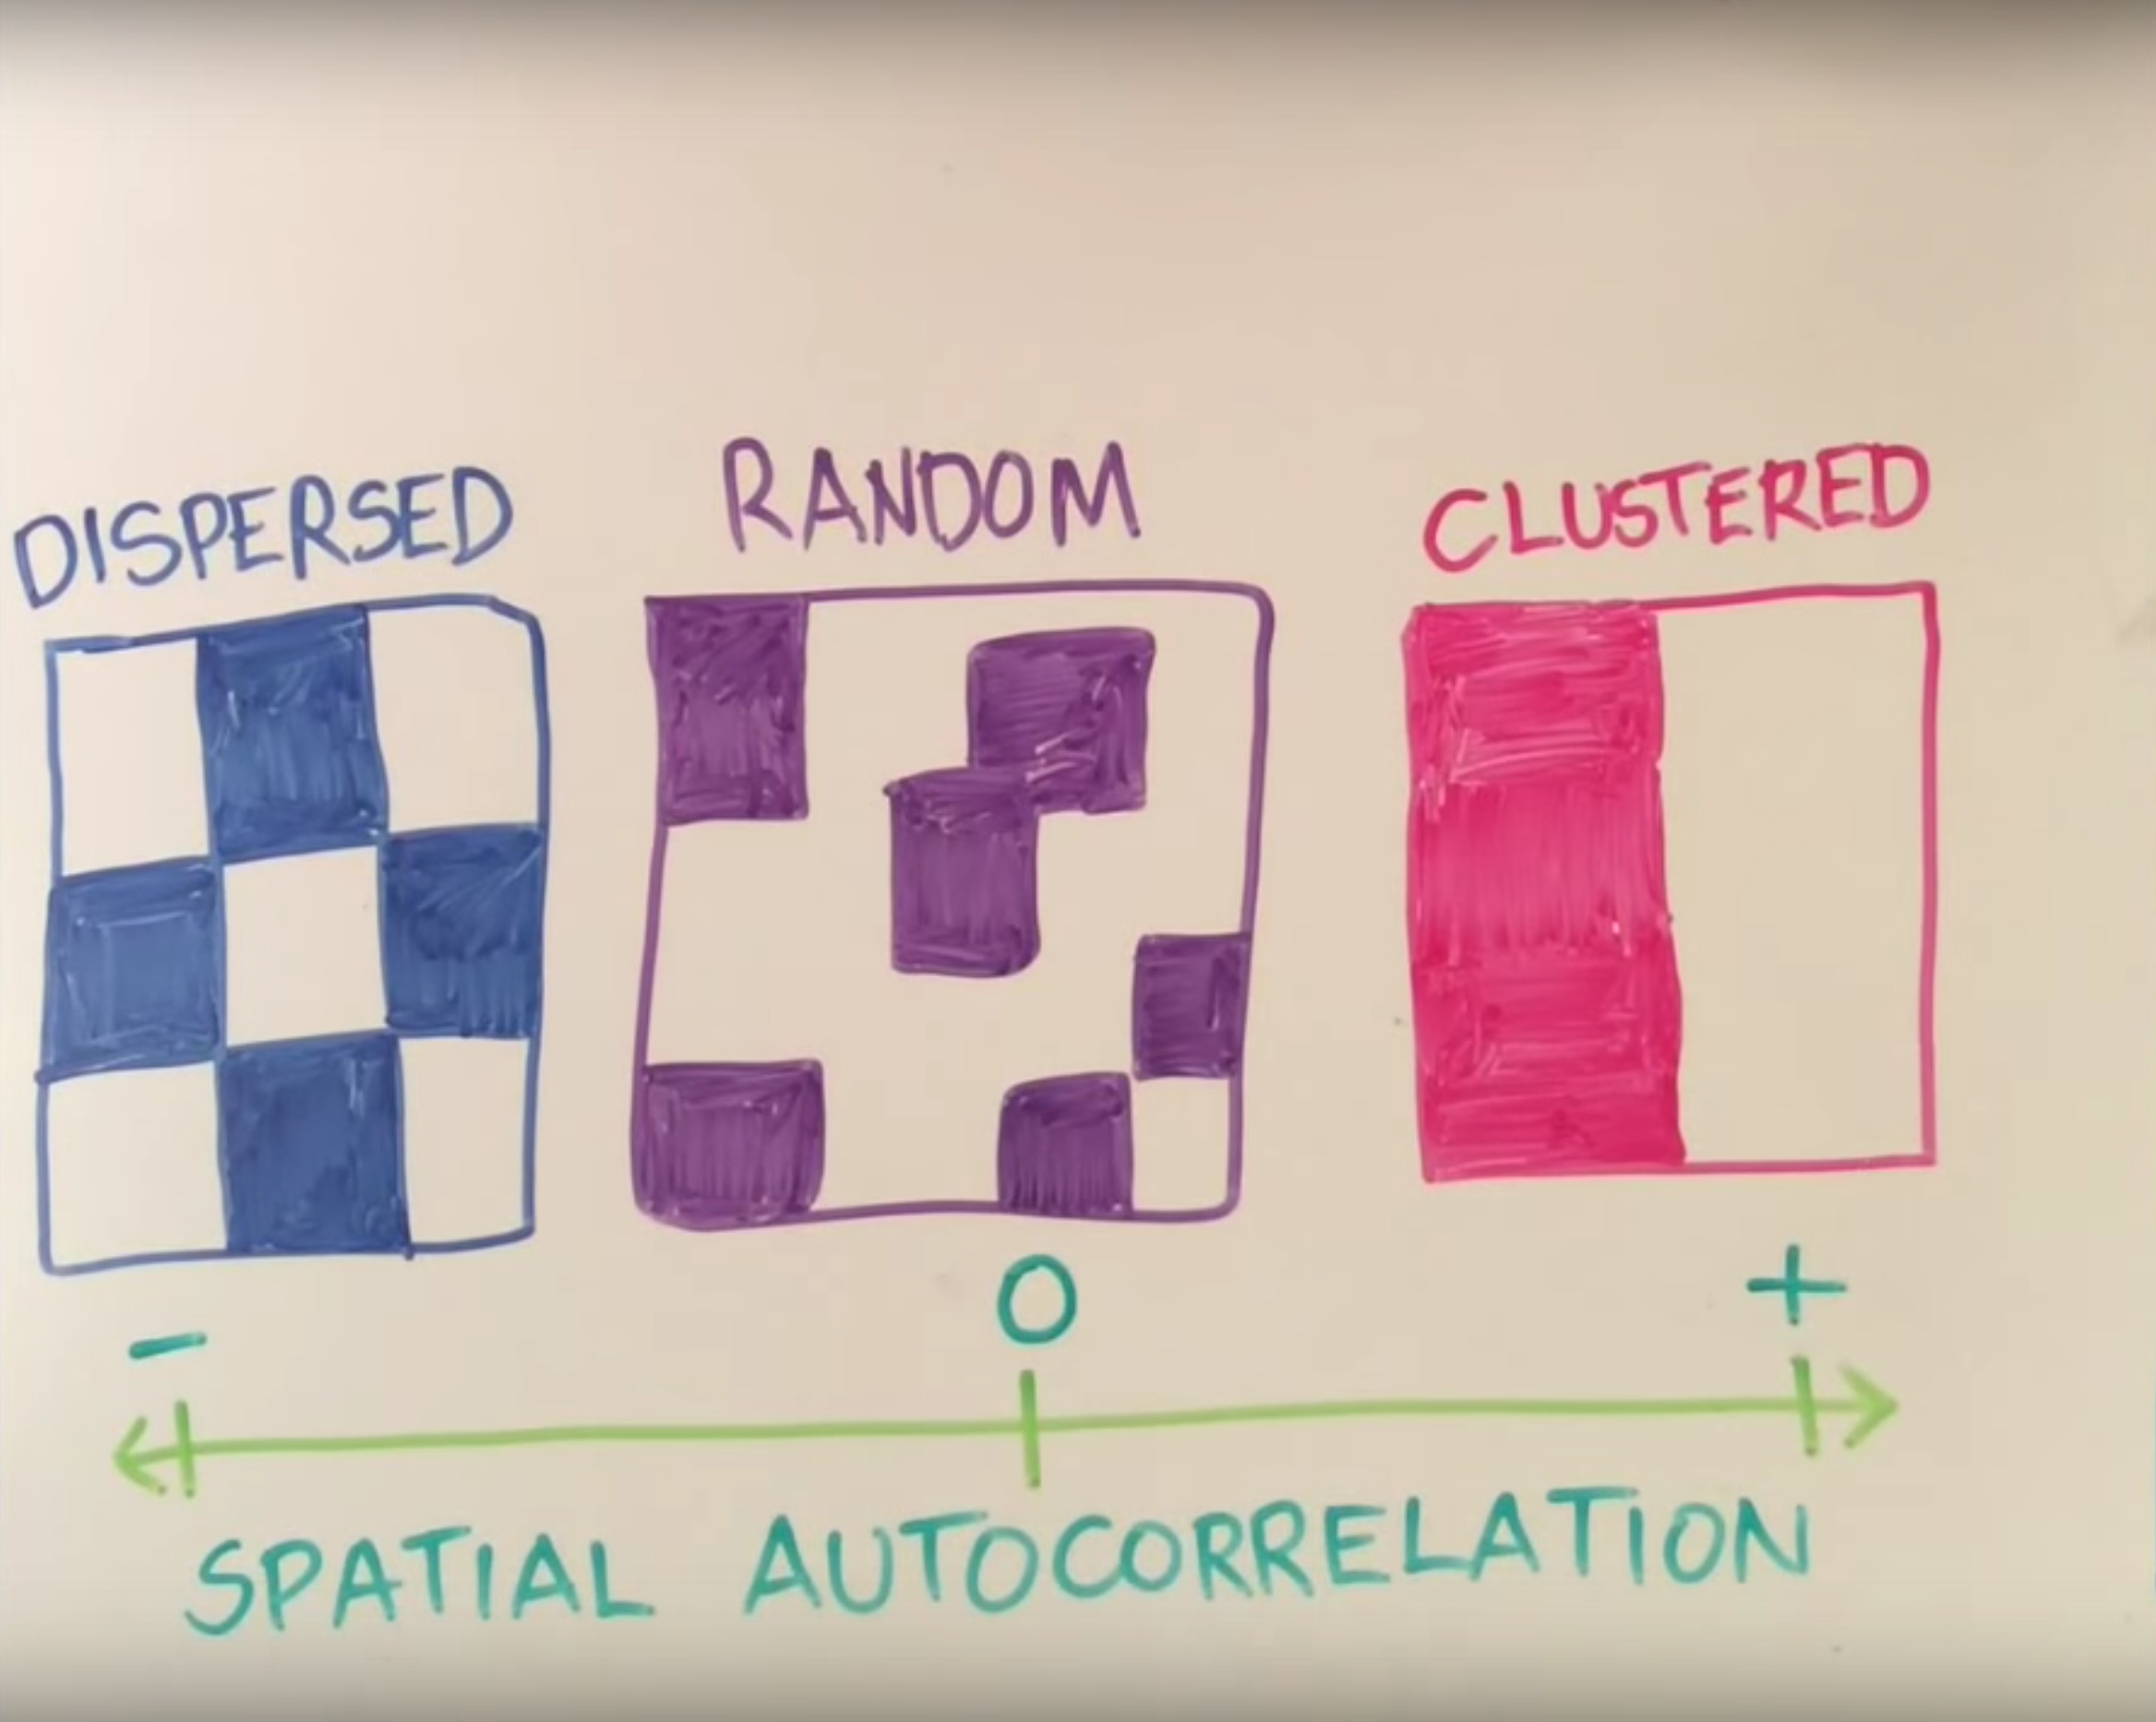
\includegraphics[width=0.8\textwidth]{autocor2}
\caption{Correlation Types}
\label{fig:autocor2}
\end{center}
\end{figure}

If an area has a high positive value then we can consider that area a hotspot. So if an area has lots of high positive values they should accumulate to generate a higher allergy symptom score. Equally, if an area has a few high positive values, a few small absolute values and a few large negative values, the algorithm should take this into account and not label the area as a hotspot.\\

An effective way of doing this is to take an average of the z-scores for the area. Then use the average in the heatmap.

\subsection{Distance Calculations}

Calculating the statistical significance of values, and whether or not they are related to nearby values involves calculating the distance between points.\\

There are many ways of calculating the distance between two dimensional points and it's not a particularly interesting topic so I'll keep it brief. I decided to use the Manhattan distance as shown below \ref{dia:manhat}.\\

$dist (x, y)  = \sqrt{\sum_{i=1}^n (x_i - y_i)^2 }$
\label{dia:manhat}

\subsection{Using distances}

The closer two points are, the more they will affect each other. It would not be correct to say that a cluster of allergy symptoms in Manchester should have any affect at all on those in Liverpool. So I need a way of using these distances to calculate how much to take the surrounding areas into account. Or as Waldo Tobler's first law of Geography puts it. "everything is related to everything else, but near things are more related than distant things." \cite{waldo}\\

As you know by now, the focus of this project is on the symptoms  of allergies. Most allergen producers do not have a method of mass dispersion. What I mean by that is they do not have a way of dispersing the produced allergens significant distances. Around 2km is normal, with the largest known distance being 21km \cite{pollenwr}. I can use this fact because I want to make sure that my hotspots are location specific and don't take into account the allergen producers over 20km because the chances are that allergens produced by them haven't reached the area.\\

The length of the entire UK is around 874 miles, with the length of the visible map in Inhale being 1000 miles. Divide this by 500 and you get 2 square miles per HotspotArray entry. This means that the average point in an area has a distance of 2 miles to the average point in the area directly to the left, right, up or down. When comparing to neighbouring areas, I want to consider the area directly next to the area in question, and maybe only very slightly consider the areas one square further than those, just to account for other types of allergens which may travel further.\\

I decided to use a inverse distance weighting with a strong fall off for neighbouring areas. See Figure \ref{table:dist} for the calculations used to determine the inverse distance function. I decided to use $\frac{1}{x^3}$ as it has the right amount of drop off for distances of 3 or more but still uses areas of distance two with a 12.5\% factor.\\ 

\begin{table}
\begin{center}
Figure \ref{table:dist} : Potential Inverse Distance Functions\\\label{table:dist}
\begin{tabular}{|c|c|c|c|}\hline\hline
x&$\mathbf{\frac{1}{x^2}}$&$\mathbf{\frac{1}{x^3}}$&$\mathbf{\frac{1}{x^4}}$\\\hline
1&1&1&1\\
2&0.25&0.125&0.0625\\
3&0.111&0.037&0123\\
4&0.0625&0.0156&0.0039\\\hline\hline
\end{tabular}
\end{center}
\end{table}


\subsection{Getis-Ord}

Getis-Ord Gi* is a spatial autocorrelation algorithm. I decided to use Getis-Ord Gi* as the alternative solutions tended not to include the feature being examined in the distance weightings. For this particular usage it is very important to include the immediate area when calculating z-scores as allergen dispersion distances are so small.

Here's the equation;

\begin{myequation}%
Gi^(*) = \frac{\sum_{j=1}^{n} w_{i,j}x_{j} - \overline{X} \sum_{j=1}^{n} w_{i,j}}{{S \sqrt{\frac{n \sum_{j=1}^{n} w^2_{i,j} - (\sum_{j=1}^{n} w_{i,j})^2}{n-1}}}}
\end{myequation}

In summary, it takes the Analysis Field and compares it to every other point on the map using the inverse distance function making sure that distant areas have less effect on the resulting value. This is then used to determine whether or not the area is locally statistically significant.

\subsection{Speed issues and the Solution}

When calculating the Getis-Ord Gi* values for each area in the 500 by 500 array, you need to calculate the distance between that area and every other area. This quickly becomes a large problem of scale $O(n^2)$. Even though the distance calculations are very fast, the total time to run the Getis-Ord calculations was 14 seconds. As Inhale is hosted online, users will be expecting a much faster, more fluid experience.\\

The Britain Breathing dataset is displayed by default every time you open the website. However, no changes are made to the data, the Getis-Ord calculations are stable so that the same input will always produce the same output so I can store the output from the Getis-Ord calculations so that I don't have to do them every time.\\

I implemented a cache system to speed up the process wherever possible. The process keeps in mind possible future updates where the user can change the base data and so is prepared to calculate the Getis-Ord calculations if necessary.\\

\begin{enumerate}
    \item Compute MD5 hash of input array
    \item Check if JSON HashMap contains an entry for the input
    \item If contains entry - pull the corresponding output array. Otherwise - compute Getis-Ord.
\end{enumerate}

When the cache finds a hit, the time taken plummets to an average over 7 runs of 120ms, a marked improvement over 14,000ms. This change was one of the simplest, but made a huge difference to the useability of Inhale.

\section{Smart Data Tool}

I display the Britain Breathing dataset and allow the user to compare it to the Road Traffic set. I would have liked to have compared to more datasets, but there are not many good, relevant geographical datasets available online. The majority cost money or are entirely private. However, this should not stop Inhale from being used by those with access to those datasets from comparing their sets to allergies.\\

I implemented a Smart Data Tool (SDT). It introduces the capability to upload your own dataset to be compared. The SDT can parse csv, tsv or JSON. For a dataset to be displayed on the map, it needs to have a location attribute. This is usually a Latitude/Longitude pair, or a Northing/Easting pair. SDT automatically detects these from the dataset and attempts to map them for you.\\

The SDT also asks for a "Value Field", this is the field that will be used as the Analysis field in representations that require hotspot identification, or it can be used as a label in datasets that only require a simple marker for each entry. For example, in Figure \ref{fig:sdt}, the uk-towns-sample.csv has automatically detected the Latitude and Longitude fields, and allows you to select an appropriate label for the marker tooltip to display when hovered over.\\

\begin{figure}[H]
\begin{center}
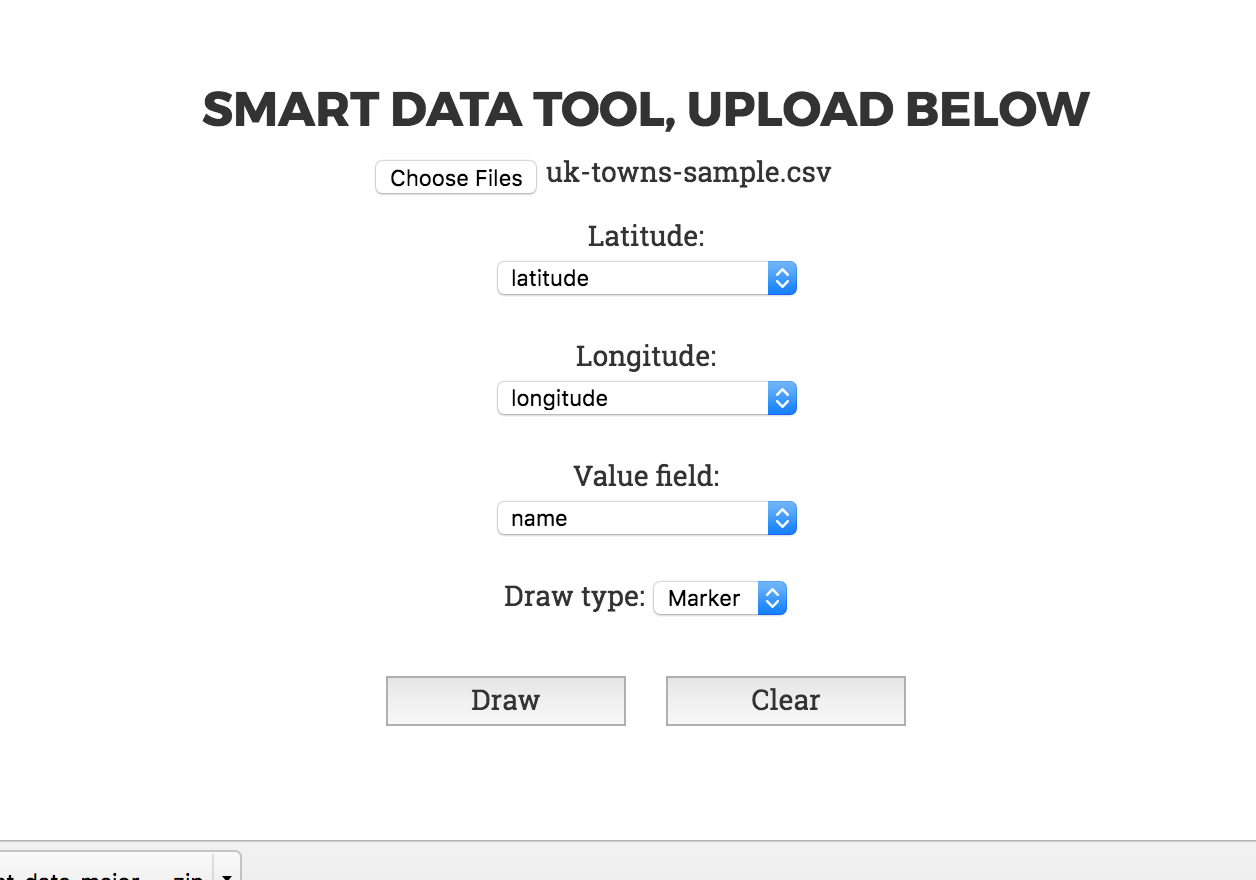
\includegraphics[width=0.4\textwidth]{sdt}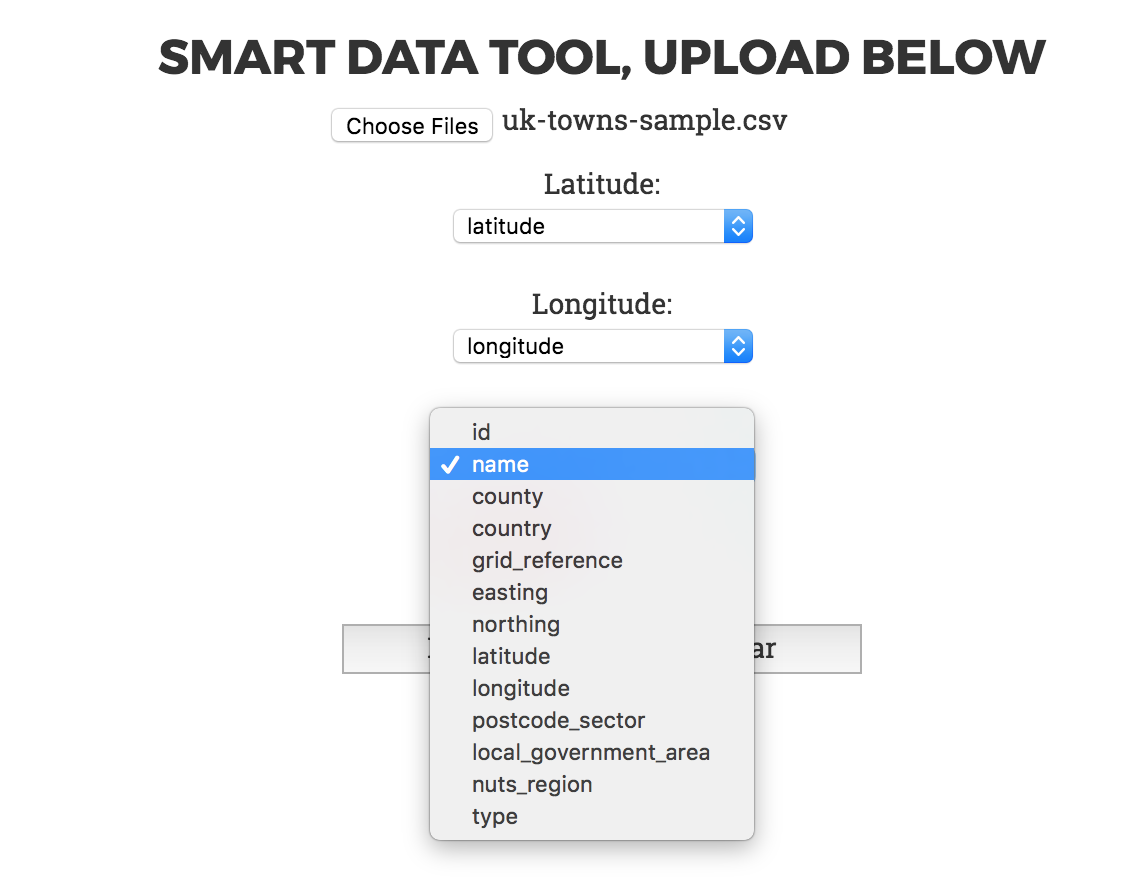
\includegraphics[width=0.4\textwidth]{sdt15}
\caption{Smart Data Tool Town Example}
\label{fig:sdt}
\end{center}
\end{figure}

And Figure \ref{fig:sdt2} shows the result when the uk-towns-sample.csv dataset is drawn with the allergy symptoms heatmap behind.

\begin{figure}[H]
\begin{center}
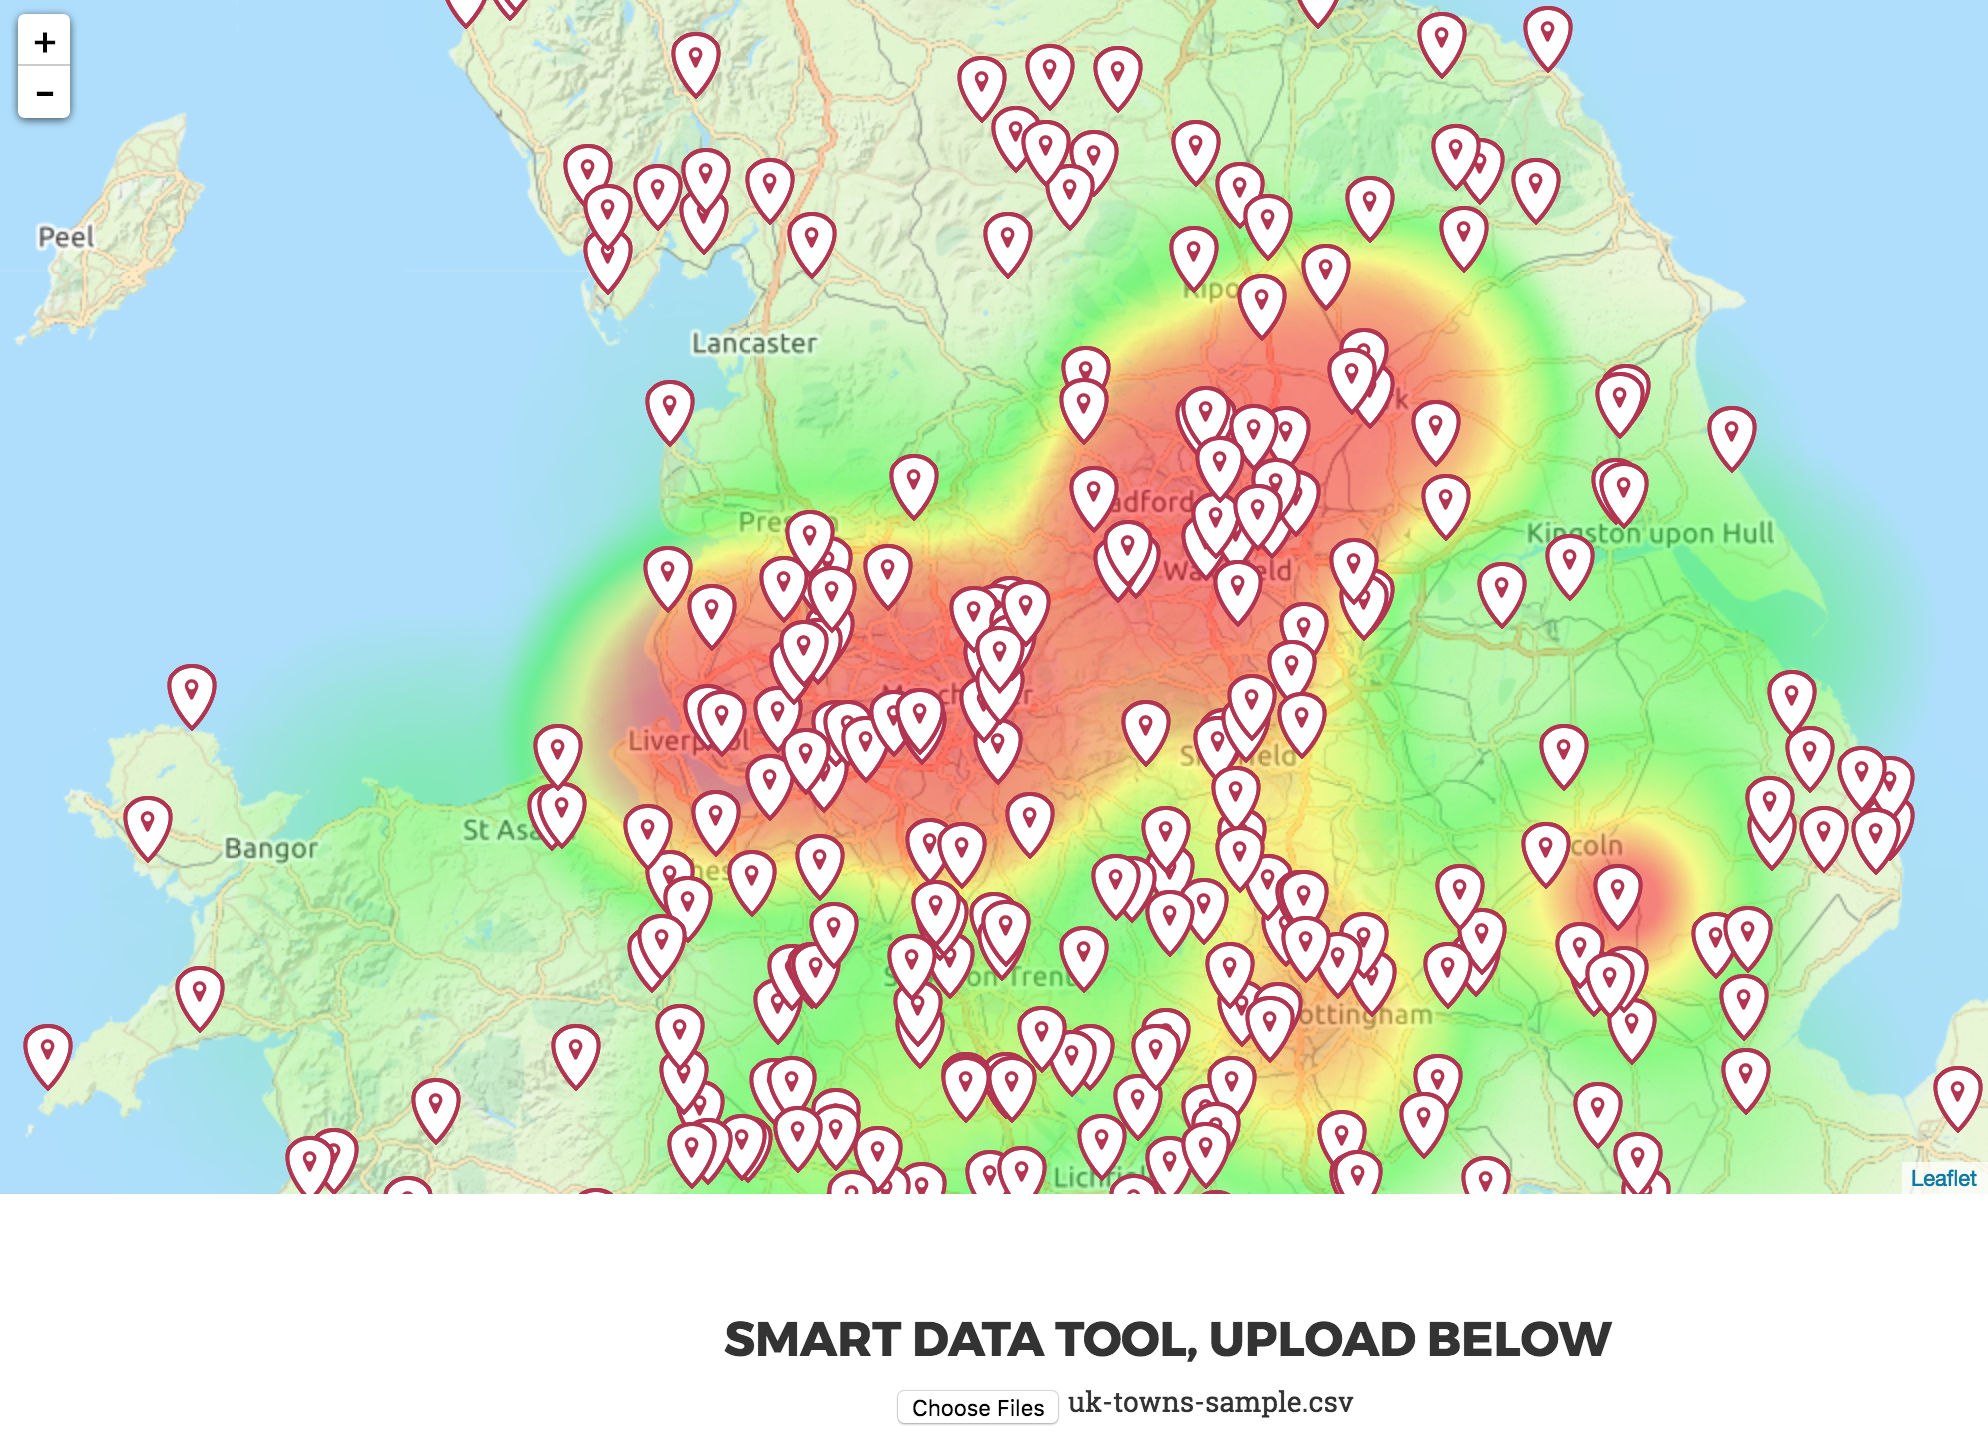
\includegraphics[width=0.4\textwidth]{sdt2}
\caption{Smart Data Tool Town Map}
\label{fig:sdt2}
\end{center}
\end{figure}